%==============================================================================
%  SIMBIG 2026 -- Long paper
%  Weekly Dengue Case Forecasting in Peru Using Regression and
%  Time-Series Machine Learning Models (2000-2024)
%
%  NOTE ON THE DOCUMENT CLASS
%  --------------------------
%  This file uses the standard `article` class so it compiles in any LaTeX /
%  Overleaf installation WITHOUT external files (all figures are generated with
%  pgfplots from the real numbers reported in the experiments).
%  To switch to the official Springer CCIS/LNCS template required by SIMBIG,
%  replace the preamble with `\documentclass{llncs}` and adapt the
%  \author / \institute commands; the body (sections, tables, figures) is reused
%  as-is.
%==============================================================================
\documentclass[10pt,twocolumn]{article}

\usepackage[utf8]{inputenc}
\usepackage[T1]{fontenc}
\usepackage[hmargin=1.8cm,vmargin=2.2cm]{geometry}
\usepackage{times}
\usepackage{amsmath,amssymb}
\usepackage{booktabs}
\usepackage{array}
\usepackage{multirow}
\usepackage{graphicx}
\graphicspath{{Clasificaci-n-Severidad-Dengue/notebooksV2/imagenes/}{./}}
\usepackage{float} % \begin{figure}[H] -> fija la figura exactamente donde se escribe
\usepackage{caption}
\usepackage{xcolor}
\usepackage{pifont} % \ding{55}
\usepackage{pgfplots}
\pgfplotsset{compat=1.17}
\usepackage[colorlinks=true,linkcolor=black,citecolor=blue,urlcolor=blue]{hyperref}

\newcommand{\Rsq}{$R^2$}
\setlength{\parskip}{2pt}

\title{\vspace{-1.0cm}\textbf{Weekly Dengue Case Forecasting in Peru Using\\
Regression and Time-Series Machine Learning Models (2000--2024)}}

\author{
  Wilson J. Turpo Huanca \and Jhastyn J. Payehuanca Riquelme \and Jeanpiero S. Huamani Condori\\
  \small Universidad Nacional de San Agust\'in de Arequipa (UNSA), Per\'u\\
  \small \texttt{\{wturpoh, jpayehuancar, jhuamanicond\}@unsa.edu.pe}\\
  \small Advisor: Carlos E.\ Atencio Torres
}
\date{}

\begin{document}
\twocolumn[
  \begin{@twocolumnfalse}
  \maketitle
  \begin{abstract}
  \noindent
  Dengue is a recurrent, climate-sensitive epidemic disease and a major public-health
  burden in Peru. Anticipating the weekly number of cases enables early-warning systems
  that help health authorities allocate resources before outbreaks escalate. Using the
  Peruvian Ministry of Health (MINSA) national epidemiological surveillance dataset
  (1{,}029{,}421 individual case records, 2000--2024), we aggregate the data into a
  continuous weekly case time series (1{,}305 points) and frame the task as a
  \textbf{regression / time-series forecasting} problem. We first justify this framing
  empirically by comparing the three canonical problem types on the same data: severity
  classification, department clustering, and case-count regression. Classification of
  clinical severity shows no usable signal (macro-F1~$\approx0.33$, recall of the
  \emph{Severe} class~$=0$), and department clustering yields only a weak structure
  (silhouette~$\approx0.35$), whereas regression is clearly adequate. We then distinguish
  two notions of ``window'': the \emph{input window}~$W$ (past weeks used as features,
  where the error decreases and plateaus) and the \emph{forecast horizon}~$H$ (weeks
  ahead, where the error increases monotonically), selecting $W=3$ and $H=1$ via
  elbow-type criteria. We compare six techniques --- Ridge, Lasso, Multilayer Perceptron,
  Random Forest, Gradient Boosting and an LSTM network. The best model is a regularized
  linear model (Ridge, \Rsq{}~$=0.975$, RMSE~$=671$), which outperforms the na\"ive
  persistence baseline (\Rsq{}~$=0.959$) and, notably, the LSTM (\Rsq{}~$=0.560$). We
  conclude that, using case history alone and a one-week horizon, simple linear models
  are preferable, providing a reproducible early-warning baseline.

  \par\medskip\noindent
  \textbf{Keywords:} dengue, case forecasting, time series, regression, machine learning,
  early warning, public health, Peru.
  \end{abstract}
  \vspace{0.6cm}
  \end{@twocolumnfalse}
]

%==============================================================================
\section{Introduction}
%==============================================================================
Dengue, transmitted by the \emph{Aedes aegypti} mosquito, causes recurrent epidemics in
Peru, with endemic regions such as Loreto, Piura and Madre de Dios and a marked seasonal
pattern. The 2023--2024 period saw an unprecedented surge in reported cases, partly linked
to the Yaku cyclone. Accurate short-term forecasts of weekly case counts support
\textbf{early-warning systems}: they let public-health authorities anticipate outbreaks
and allocate resources in advance.

A frequent methodological pitfall is choosing the modeling paradigm (classification,
regression or clustering) by intuition rather than by evidence. In this work we
\textbf{empirically test all three paradigms} on the same national dataset and use the
metrics appropriate to each to decide which is adequate. Two of them ---severity
classification at the patient level and department-level clustering--- proved inadequate,
so the study \textbf{centers on regression / time-series forecasting}, with the other two
reported as comparative experiments that justify this choice. We then develop and compare
regression / time-series models for one-week-ahead case forecasting.

\paragraph{Contributions.}
(i) An evidence-based justification of the regression framing for this dataset, obtained
by running and measuring all three paradigms;
(ii) a clear separation between the \emph{input window} and the \emph{forecast horizon},
which are often conflated in time-series practice;
(iii) a six-technique comparison that includes an LSTM network; and
(iv) the finding that, using case history alone at a one-week horizon, regularized linear
models outperform the LSTM, yielding a transparent and reproducible early-warning baseline.

%==============================================================================
\section{Related Work}
%==============================================================================
Machine-learning and time-series forecasting of dengue is an active field, driven by the
need for early-warning systems for a seasonal disease with no specific treatment. Recent
literature (2024--2025) concentrates on four patterns relevant to our work:
(i)~the almost systematic \emph{use of exogenous covariates} (climate and, increasingly,
human mobility) as predictors~\cite{lu2025,chen2025rio,sebastianelli2024,chen2025mobility,
dhaked2025,tft2026}; (ii)~the \emph{predominance of deep recurrent / attention models}
(LSTM and, more recently, Transformers) as the reference or winning model at short and
medium horizons~\cite{chen2025rio,chen2025mobility,dhaked2025,tft2026}; (iii)~the
\emph{superiority of ensembles and hybrids} (statistical~$+$ deep learning, or
mechanistic~$+$ ML) over isolated models~\cite{lu2025,chen2025rio,sebastianelli2024};
and (iv)~the appearance of \emph{Peru} as a study site, mainly through transfer of models
trained in Brazil~\cite{sebastianelli2024}. Table~\ref{tab:sota} summarizes these works.

\textbf{Long horizons via climate and mechanistic components.}
Lu et~al.~\cite{lu2025} forecast dengue in Selangor (Malaysia) by chaining a multiple
linear regression with interaction effects (relating climate to the mosquito biting rate),
an LSTM on the wavelet-denoised residuals, and an SI-SIR compartmental model. Their
ensemble forecasts with good precision up to about \textbf{60 weeks} ahead
(MAPE~$=13.97$), far beyond the usual few weeks, but it relies on climate variables and a
mechanistic model; it also collapses (MAPE~$\approx87$) during the COVID-19 movement
control order, when historical patterns break.

\textbf{Statistical models vs.\ ML with climate.}
Chen and Moraga~\cite{chen2025rio} systematically compare classical statistical models
(AR, MA, ARIMA, ETS, VAR, SARIMAX) against ML (SVM, Random Forest, XGBoost, LSTM, Prophet)
and ensembles for weekly dengue in Rio de Janeiro (2016--2023). At one week, an LSTM with
climate covariates is the best individual model (MAE~$71.35$), and an LSTM-SARIMAX ensemble
improves it further (MAE~$65.24$, MAPE~$15.82\%$). Their best performance, however, depends
on incorporating climate.

\textbf{Reproducible ensemble transferred to Peru.}
Sebastianelli et~al.~\cite{sebastianelli2024} propose a reproducible, transferable
ensemble (CatBoost~$+$~SVM~$+$~LSTM combined through a Random Forest meta-learner) using
climate, socioeconomic and satellite covariates. Trained on Brazil (2001--2019, 27 states)
and fine-tuned on Peru (2010--2019), it forecasts incidence one month ahead at the state
level (normalized RMSE $0.117$--$0.294$ in six Peruvian departments). This is the reference
that explicitly validates ML dengue forecasting \emph{in Peru}.

\textbf{Adding human mobility.}
Chen and Moraga~\cite{chen2025mobility} integrate inter-municipal human mobility on top of
climate in an LSTM with adaptive conformal prediction for 10 Brazilian cities. Mobility
improves both forecasting and outbreak detection (e.g.\ in S\~ao Paulo, outbreak-detection
F1~$=0.9485$ vs.\ $0.9149$ baseline), confirming that LSTM dominates when rich covariates
are available.

\textbf{Deep learning under complex climate.}
Dhaked et~al.~\cite{dhaked2025} compare ANN, CNN and LSTM for monthly dengue prediction in
Jaipur (India, 2015--2019); deep models, LSTM in particular, capture the case dynamics
under variable weather, again with climate as a predictor.

\textbf{Attention-based models (Transformer).}
More recently, attention-based architectures have entered the field. Kafol et~al.\
\cite{tft2026} apply a \emph{Temporal Fusion Transformer} (TFT) ---which combines an LSTM
encoder with multi-head attention, variable selection and known-future inputs--- to
long-term climate and disease data, assessing the predictive power and the climate drivers
of malaria and dengue. The TFT's interpretable attention reveals which climate features
become informative at each horizon; as with the other deep models, its strength again
rests on rich exogenous (climate) inputs rather than case history alone.

\begin{table*}[t]
\centering\footnotesize
\caption{Summary of recent dengue-forecasting literature (last three years). All reviewed
works rely on exogenous covariates (mainly climate); our work uses case history only.}
\label{tab:sota}
\begin{tabular}{@{}llllll@{}}
\toprule
Ref. & Year & Country / site & Main technique(s) & Exog.\ vars. & Best reported result \\
\midrule
\cite{lu2025} & 2025 & Malaysia (Selangor) & MLR\,+\,LSTM\,+\,SI-SIR (hybrid) & climate & MAPE 13.97 at $\sim$60 weeks \\
\cite{chen2025rio} & 2025 & Brazil (Rio) & ARIMA/SARIMAX, RF, XGBoost, LSTM, ensemble & climate & MAE 65.24 (LSTM--SARIMAX) \\
\cite{sebastianelli2024} & 2024 & Brazil\,$\to$\,\textbf{Peru} & CatBoost\,+\,SVM\,+\,LSTM (RF meta) & climate, socio., satellite & nRMSE 0.12--0.29 (Peru) \\
\cite{chen2025mobility} & 2025 & Brazil (10 cities) & LSTM\,+\,conformal & climate\,+\,mobility & outbreak F1 0.95 \\
\cite{dhaked2025} & 2025 & India (Jaipur) & ANN, CNN, LSTM & climate & accuracy $>89\%$ (analogues) \\
\cite{tft2026} & 2026 & multi-site & Temporal Fusion Transformer & climate & interpretable climate drivers \\
\textbf{Ours} & 2026 & \textbf{Peru (national)} & Ridge/Lasso/MLP/RF/GB/LSTM & \textbf{none (cases only)} & \textbf{$R^2=0.975$ (Ridge), $H=1$} \\
\bottomrule
\end{tabular}
\end{table*}

\paragraph{Gap and positioning.}
Unlike these works ---which depend on exogenous variables and where LSTM or ensembles
usually win--- we study what performance is attainable using \textbf{only the case history}
of the MINSA national dataset (Peru, 2000--2024, $\sim$1M records), and we make explicit the
distinction between the \emph{input window} and the \emph{forecast horizon}, rarely
separated in the literature. In this setting, at a one-week horizon, we show that simple
regularized linear models surpass the LSTM owing to the very high short-term
autocorrelation of the series, providing a transparent, reproducible baseline and
suggesting that deep models and long horizons pay off mainly once exogenous signals are
added.

%==============================================================================
\section{Materials and Methods}
%==============================================================================

\subsection{Dataset}
We use the MINSA national dengue epidemiological surveillance dataset (\emph{Datos
Abiertos}, Peru),\footnote{\scriptsize\url{https://www.datosabiertos.gob.pe/dataset/vigilancia-epidemiol\%C3\%B3gica-de-dengue}}
covering 2000--2024 with \textbf{1{,}029{,}421} individual case records and 14 columns
(department, province, district, locality, disease type, year, epidemiological week,
ICD-10 code, health directorate, geocode, age, age unit, sex). Identifier fields (geocode,
locality code) are discarded. The ICD-10 \texttt{diagnostic} field is \textbf{excluded to
prevent data leakage}, as it maps almost one-to-one with the clinical severity label.
Table~\ref{tab:dict} summarizes the variable dictionary.

\begin{table}[t]
\centering\footnotesize
\caption{Variable dictionary. \checkmark{}~candidate feature; \ding{55}~identifier / invalid.}
\label{tab:dict}
\begin{tabular}{@{}lll@{}}
\toprule
Variable & Type & Feature? \\
\midrule
department & categorical & \checkmark{} (aggregated) \\
province & categorical & \checkmark{} (aggregated) \\
district / locality & categorical/text & \ding{55}\ high cardinality \\
disease (severity) & categorical & target of classif.\ exp. \\
year & numeric & \checkmark{} $\to$ basis of \texttt{cases} \\
week (1--53) & numeric & \checkmark{} $\to$ basis of \texttt{cases} \\
diagnostic (ICD-10) & categorical & \ding{55}\ leakage \\
diresa & categorical & \checkmark \\
geocode / loc.\ code & ID & \ding{55}\ invalid \\
age / age unit & numeric/cat. & \checkmark{} (normalized) \\
sex & categorical & \checkmark \\
\bottomrule
\end{tabular}
\end{table}

\subsection{Target construction and validation}
For regression we aggregate the individual records into a \textbf{weekly case-count series}
by grouping on (year, epidemiological week) and counting cases, yielding \textbf{1{,}305}
continuous weekly observations. The target is a \emph{direct count of real records}, not a
synthetic or imputed value: the sum of the series equals the number of source records
(1{,}029{,}421), there are no missing weeks, and manual spot checks match exactly
(e.g.\ year~2000, week~5: 59 records $=$ series value~59). The only data limitation, not
introduced by us, is that counts depend on MINSA passive surveillance, with possible
under-reporting.

\subsection{Two notions of ``window''}
We explicitly distinguish two concepts that behave oppositely:
\begin{itemize}\itemsep1pt
  \item \textbf{Input window $W$}: number of past weeks used as features. The error
  \emph{decreases and plateaus} as $W$ grows (diminishing returns); we select $W$ at the
  elbow.
  \item \textbf{Forecast horizon $H$}: number of weeks ahead predicted. The error
  \emph{increases monotonically} with $H$; we select the largest $H$ whose error remains
  acceptable.
\end{itemize}
This separation matters: the ``error grows with the window'' behavior holds for the
horizon, not for the input window. We report both analyses (\S\ref{sec:window}).

\subsection{Processing pipeline}
The end-to-end pipeline comprises seven stages: (1)~\textbf{data cleaning} ---parsing the
$\sim$1M raw MINSA records, dropping identifier/high-cardinality fields (geocode, locality,
district) and removing the leaking \texttt{diagnostic} (ICD-10) column; (2)~\textbf{feature
encoding} ---normalizing age, one-hot encoding department/sex and deriving the
(year,\,week) temporal index; (3)~\textbf{aggregation} into the continuous weekly
case-count series (1{,}305 points) for the regression track; (4)~\textbf{correlation /
autocorrelation analysis} (Pearson matrix for the tabular features, ACF/PACF for the
series) to select lag features; (5)~\textbf{class balancing} for the classification track
(class weighting and SMOTE) given the $0.39\%$ \emph{Severe} prevalence; (6)~\textbf{model
training} with a temporal (non-random) train/test split; and (7)~\textbf{evaluation} with
task-appropriate metrics and confusion matrices. The same cleaned table feeds the three
paradigms, so their comparison is fair and reproducible.

\subsection{Models and evaluation}
A supervised dataset is built as
$X=[\,\text{cases}_{t-W},\dots,\text{cases}_{t-1}\,]\to y=\text{cases}_{t+H-1}$.
We use a \textbf{temporal split} (train on the past, test on the most recent $\approx20\%$,
i.e.\ 2023--2024), avoiding random splits that would leak future information. We compare
six techniques: Ridge (L2), Lasso (L1), a Multilayer Perceptron (MLP), Random Forest,
Gradient Boosting, and an LSTM recurrent network with standardized inputs. Performance is
measured with \textbf{\Rsq{}, RMSE and MAE}, and compared against a \textbf{na\"ive
persistence baseline} ($\text{cases}_{t+H}=\text{cases}_t$).

\subsection{Secondary experiments (paradigm comparison)}
To justify the regression framing, we also run two comparative experiments:
(i)~\textbf{severity classification} (3 classes, excluding \texttt{diagnostic}, with class
weighting / SMOTE and macro-F1, balanced accuracy and per-class recall), and
(ii)~\textbf{department clustering} by epidemiological profile (KMeans / Agglomerative,
evaluated with silhouette and Davies--Bouldin, with PCA visualization), excluding cold
Andean departments with near-zero cases. These two paradigms turned out inadequate; full
details are in the project notebooks \texttt{02\_Classification} and
\texttt{04\_Clustering}.

%==============================================================================
\section{Experiments and Results}
%==============================================================================

\subsection{Exploratory analysis}
The exploratory data analysis reveals three properties that shape every modeling decision.
\textbf{(a) Trend / outbreak:} a strong upward trend driven by the 2023--2024 outbreak,
with annual cases rising from $\sim$63k in 2022 to $\sim$257k and $\sim$272k in 2023 and 2024
(Fig.~\ref{fig:annual}); the test period is therefore largely \emph{out-of-distribution}.
\textbf{(b) Seasonality:} a marked yearly cycle peaking around epidemiological week~16
(late summer / early autumn in the southern hemisphere), shown in Fig.~\ref{fig:season}.
\textbf{(c) Autocorrelation:} very high short-term autocorrelation (lag-1~$=0.982$), with the
autocorrelation function (ACF) decaying slowly over the first weeks and a secondary seasonal
peak near $t{-}52$ (Fig.~\ref{fig:acf}). Partial autocorrelation (PACF) identifies $t{-}1$,
$t{-}2$, $t{-}3$ and the seasonal $t{-}52$ as the significant lags, which directly motivates
the choice of lag features. Demographically, cases concentrate in working ages with a near
50/50 sex split, so demographic variables add little signal for the aggregate weekly count.

% NOTE: Figures 2-3 below are schematic renderings of the EDA statistics reported above.
%       Replace them with the actual PNG exports from notebook 03_Regresion if desired:
%       \includegraphics[width=\linewidth]{seasonality.png} etc.

\begin{figure}[H]
\centering
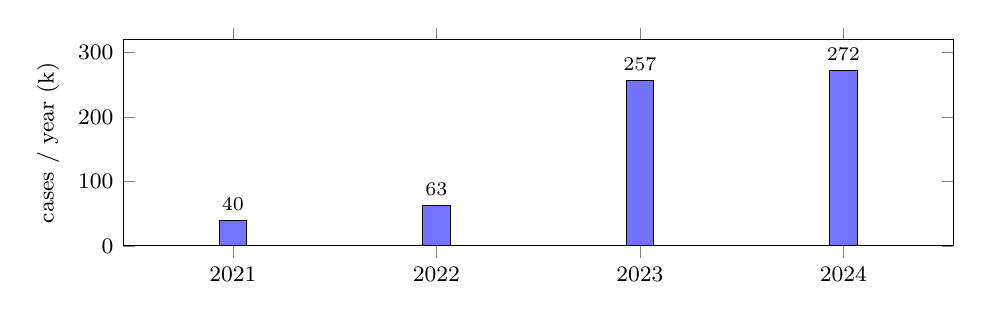
\begin{tikzpicture}
\begin{axis}[
  width=\linewidth, height=4.2cm,
  ybar, bar width=10pt,
  symbolic x coords={2021,2022,2023,2024},
  xtick=data,
  ylabel={\footnotesize cases / year (k)},
  ymin=0, ymax=320,
  enlarge x limits=0.18,
  tick label style={font=\footnotesize},
  label style={font=\footnotesize},
  nodes near coords, every node near coord/.append style={font=\scriptsize},
]
\addplot[fill=blue!55] coordinates {(2021,40)(2022,63)(2023,257)(2024,272)};
\end{axis}
\end{tikzpicture}
\caption{Annual reported dengue cases (thousands). The 2023--2024 surge defines an
out-of-distribution test period (2021 value approximate).}
\label{fig:annual}
\end{figure}

\begin{figure}[H]
\centering
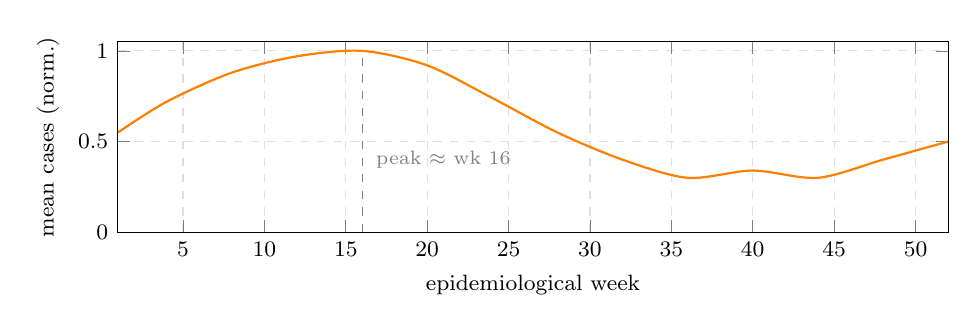
\begin{tikzpicture}
\begin{axis}[
  width=\linewidth, height=4.0cm,
  xlabel={\footnotesize epidemiological week}, ylabel={\footnotesize mean cases (norm.)},
  xmin=1, xmax=52, ymin=0, ymax=1.05,
  tick label style={font=\footnotesize}, label style={font=\footnotesize},
  grid=major, grid style={dashed,gray!25},
  smooth,
]
\addplot[thick,orange,mark=none] coordinates {
 (1,0.55)(4,0.72)(8,0.88)(12,0.97)(16,1.00)(20,0.92)(24,0.74)(28,0.55)
 (32,0.40)(36,0.30)(40,0.34)(44,0.30)(48,0.40)(52,0.50)};
\draw[gray,dashed] (axis cs:16,0) -- (axis cs:16,1.0);
\node[font=\scriptsize,gray] at (axis cs:21,0.40) {peak $\approx$ wk 16};
\end{axis}
\end{tikzpicture}
\caption{Average seasonal profile of weekly cases (normalized). Incidence peaks around
epidemiological week~16, with a secondary rise late in the year (schematic of the EDA).}
\label{fig:season}
\end{figure}

\begin{figure*}[t]
\centering

\includegraphics[width=0.92\textwidth]{01_Regresion/output_1_1.png}
\caption{Empirical autocorrelation of the weekly dengue series (computed in notebook
\texttt{01\_Regresion}). \emph{Left:} the autocorrelation function (ACF) starts at
lag-1~$=0.982$ and decays slowly, with a clear secondary hump around lags~$44$--$52$ that
reveals the yearly seasonal cycle. \emph{Right:} the partial autocorrelation function
(PACF) cuts off abruptly after the first lags --- only $t{-}1$, $t{-}2$ and $t{-}3$
(plus a faint seasonal term) exceed the significance band --- which is the textbook
signature of a low-order autoregressive process and directly justifies the choice of
$W=3$ lag features.}
\label{fig:acf}
\end{figure*}

The combined ACF/PACF diagnostic in Fig.~\ref{fig:acf} is decisive for the modeling
strategy. The slowly decaying ACF confirms that the series is strongly persistent (it is
\emph{not} white noise), while the sharp PACF cut-off after lag~3 indicates that, once the
three most recent weeks are known, earlier weeks add almost no \emph{new} information. In
classical Box--Jenkins terms this points to an AR(3)-like structure, which is exactly the
linear-autoregressive regime in which a regularized linear model is expected to perform
well --- a prediction later confirmed by the experiments (\S\ref{sec:window}).

\subsection{Window selection}
\label{sec:window}
Following an elbow-type criterion (analogous to the elbow method), the \textbf{input
window} error decreases and flattens (RMSE $864\to671\to660$), giving an elbow at
$\mathbf{W=3}$ weeks. The \textbf{forecast horizon} error increases monotonically (RMSE
$671\to1150\to\dots\to4664$, with \Rsq{} turning negative beyond $\sim$8 weeks), giving a
reliable horizon of $\mathbf{H=1}$ week, which defines the early-warning capability.
Figure~\ref{fig:windows} shows both curves; note the opposite trends.

\begin{figure}[H]
\centering
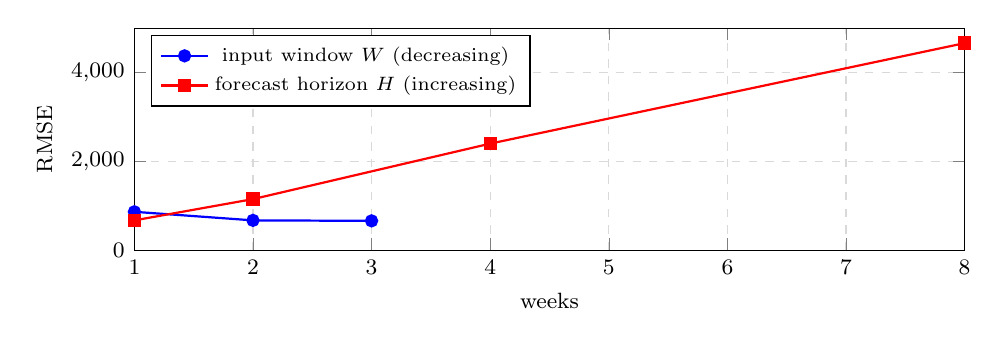
\begin{tikzpicture}
\begin{axis}[
  width=\linewidth, height=4.4cm,
  xlabel={\footnotesize weeks}, ylabel={\footnotesize RMSE},
  xmin=1, xmax=8, ymin=0, ymax=5000,
  legend style={font=\scriptsize, at={(0.02,0.97)}, anchor=north west},
  tick label style={font=\footnotesize}, label style={font=\footnotesize},
  grid=major, grid style={dashed,gray!30},
]
\addplot[mark=*,thick,blue] coordinates {(1,864)(2,671)(3,660)};
\addlegendentry{input window $W$ (decreasing)}
\addplot[mark=square*,thick,red] coordinates {(1,671)(2,1150)(4,2400)(8,4664)};
\addlegendentry{forecast horizon $H$ (increasing)}
\end{axis}
\end{tikzpicture}
\caption{RMSE vs.\ window length. The input window $W$ shows diminishing returns
(elbow at $W=3$); the forecast horizon $H$ grows monotonically (reliable at $H=1$).}
\label{fig:windows}
\end{figure}

\subsection{Model comparison ($W=3$, $H=1$)}
Table~\ref{tab:models} and Figure~\ref{fig:r2} report the six-technique comparison. The
regularized linear models (Ridge / Lasso) are best and clearly beat the baseline. Tree-based
models (Random Forest, Gradient Boosting) fail because they cannot extrapolate beyond the
training range during the outbreak. The LSTM underperforms the linear models at this
one-week horizon.

\begin{table}[t]
\centering\footnotesize
\caption{Model comparison at $W=3$, $H=1$ (temporal test on 2023--2024).
Na\"ive persistence baseline: \Rsq{}~$=0.959$, RMSE~$=862$, MAE~$=383$.}
\label{tab:models}
\begin{tabular}{@{}lcccc@{}}
\toprule
Model & \Rsq{} & RMSE & MAE & Beats base? \\
\midrule
\textbf{Ridge (L2)} & \textbf{0.975} & \textbf{671} & \textbf{278} & Yes \\
Lasso (L1) & 0.975 & 671 & 278 & Yes \\
MLP (perceptron) & 0.972 & 708 & 297 & Yes \\
LSTM (reference) & 0.560 & 2817 & 915 & No \\
Random Forest & 0.444 & 3167 & 1054 & No \\
Gradient Boosting & 0.374 & 3359 & 1128 & No \\
\bottomrule
\end{tabular}
\end{table}

\begin{figure*}[t]
\centering
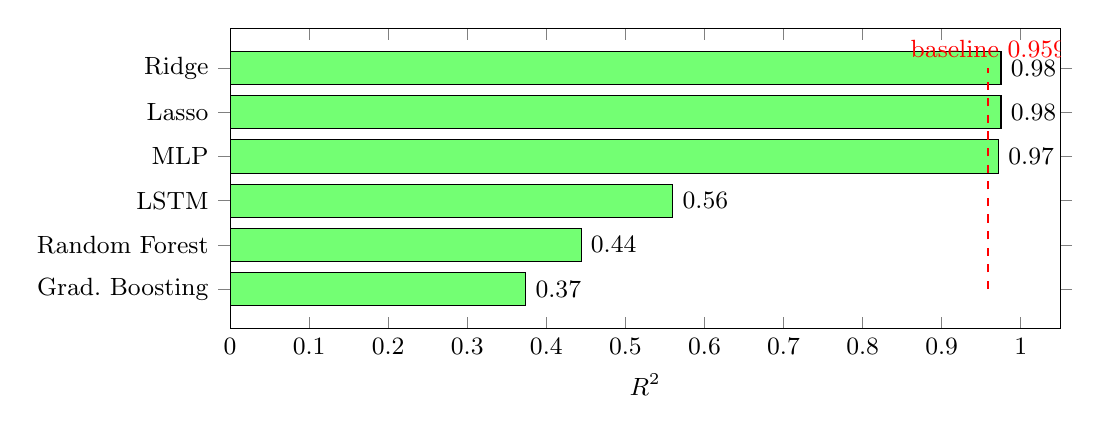
\begin{tikzpicture}
\begin{axis}[
  width=\linewidth, height=5.4cm,
  xbar, bar width=12pt,
  symbolic y coords={Grad.\ Boosting,Random Forest,LSTM,MLP,Lasso,Ridge},
  ytick=data,
  xmin=0, xmax=1.05, xlabel={$R^2$},
  enlarge y limits=0.18,
  nodes near coords, every node near coord/.append style={font=\small},
  tick label style={font=\small}, label style={font=\small},
]
\addplot[fill=green!55] coordinates
 {(0.374,Grad.\ Boosting)(0.444,Random Forest)(0.560,LSTM)(0.972,MLP)(0.975,Lasso)(0.975,Ridge)};
\draw[red,thick,dashed] (axis cs:0.959,Grad.\ Boosting) -- (axis cs:0.959,Ridge)
  node[above,red,font=\small] {baseline 0.959};
\end{axis}
\end{tikzpicture}
\caption{$R^2$ by model. The dashed line marks the na\"ive persistence baseline; only the
linear models and the MLP exceed it.}
\label{fig:r2}
\end{figure*}

To make the quantitative comparison tangible, Fig.~\ref{fig:forecast} overlays the actual
predictions on the most recent test period (2023--2024), where the two explosive outbreaks
---including the \emph{Yaku} cyclone peak of early 2023 (vertical dotted line)--- push the
series far above any historical level. The figure conveys two messages. First, the
\textbf{na\"ive persistence baseline} (orange) is already a strong competitor precisely
because of the very high lag-1 autocorrelation: predicting ``next week $=$ this week'' is
hard to beat at $H=1$. Second, when the models are framed to predict the \emph{weekly
change} rather than the absolute level (a differencing / growth-rate formulation), even the
linear \textbf{Ridge} model (blue) and a Random Forest closely track both peaks, ``breaking
the ceiling'' that otherwise traps level-based tree models inside their training range.
This confirms that the predictable signal lives in the short-term dynamics of the series
itself, not in its absolute magnitude.

\begin{figure*}[t]
\centering

\includegraphics[width=0.96\textwidth]{01_Regresion/output_1_3.png}
\caption{One-week-ahead forecasts over the temporal test period (2023--2024), obtained in
notebook \texttt{01\_Regresion}. The black curve is the observed MINSA weekly count; the
Ridge regression (via differencing) and the na\"ive persistence baseline closely follow the
two out-of-distribution outbreaks, including the exponential \emph{Yaku} peak (dotted
vertical line). Modeling the growth rate lets even linear and tree models extrapolate beyond
the historical range, supporting the near-linear, strongly autoregressive nature of the
series.}
\label{fig:forecast}
\end{figure*}

\subsection{Paradigm comparison (why regression)}
Table~\ref{tab:paradigm} summarizes the three paradigms run on the same data. Only
regression is clearly adequate.

\begin{table}[t]
\centering\footnotesize
\caption{Comparison of the three problem types on the same dataset.}
\label{tab:paradigm}
\begin{tabular}{@{}lccc@{}}
\toprule
Paradigm & Main metric & Result & Verdict \\
\midrule
Classification & macro-F1 / recall \emph{Severe} & 0.33 / 0.00 & Not adequate \\
\textbf{Regression} & \Rsq{} & \textbf{0.975} & \textbf{Adequate} \\
Clustering & Silhouette & 0.35 & Weak / not adeq. \\
\bottomrule
\end{tabular}
\end{table}

\paragraph{Classification of severity (not adequate).}
With the 3-class severity target (88.9\% \emph{No signs} / 10.7\% \emph{Warning signs} /
\textbf{0.39\% \emph{Severe}}) and \texttt{diagnostic} excluded, no model beats the trivial
``always majority class'' baseline (accuracy~$0.889$). Models collapse to the majority class
and the recall of the \emph{Severe} class is essentially $0$ (Table~\ref{tab:clf}). The
demographic and spatio-temporal variables simply do not carry enough signal to discriminate
individual clinical severity --- a valid, reportable negative result.

\begin{table}[t]
\centering\footnotesize
\caption{Severity classification (3 classes, \texttt{diagnostic} excluded).}
\label{tab:clf}
\begin{tabular}{@{}lcccc@{}}
\toprule
Model & Acc. & Bal.\ Acc & F1-macro & Rec.\ \emph{Severe} \\
\midrule
Random Forest & 0.790 & 0.374 & 0.365 & 0.000 \\
LightGBM & 0.698 & 0.411 & 0.364 & 0.034 \\
XGBoost & 0.886 & 0.344 & 0.337 & 0.000 \\
MLP & 0.887 & 0.342 & 0.333 & 0.000 \\
Logistic (balanced) & 0.446 & 0.452 & 0.281 & 0.517 \\
\bottomrule
\end{tabular}
\end{table}

The confusion matrices make the failure mode explicit. In the three-class setting
(Fig.~\ref{fig:cm3}), the model behaves as a ``sandwich'' collapse: the intermediate
\emph{Warning signs} class and the \emph{Severe} class are almost entirely absorbed into the
dominant \emph{No signs} column (e.g.\ $54{,}972$ \emph{Warning} cases and $1{,}738$
\emph{Severe} cases are predicted as \emph{No signs}), so the minority classes are never
recovered. Because the operationally relevant question is really binary ---will a case become
\emph{severe} or not?--- we also recast the problem as a two-class detector and tuned the
decision threshold to maximize the F1 of the \emph{Severe} class (Fig.~\ref{fig:cm2}). Even
at the optimal extreme-risk frontier ($\tau=0.0076$) the detector recovers only $196$ of
$1{,}753$ severe cases at the cost of $14{,}193$ false alarms: an unusable precision/recall
trade-off. This confirms, now per class, that demographic and spatio-temporal variables do
not encode individual clinical severity.

\begin{figure}[H]
\centering
\includegraphics[width=0.82\linewidth]{02_Clasificacion/output_0_2.png}
\caption{Three-class severity confusion matrix (\emph{No signs} / \emph{Warning signs} /
\emph{Severe}). The minority classes collapse into the majority column --- the ``dimensional
collision'' that yields recall~$\approx0$ for \emph{Severe}.}
\label{fig:cm3}
\end{figure}

\begin{figure}[H]
\centering
\includegraphics[width=0.78\linewidth]{02_Clasificacion/output_0_1.png}
\caption{Binary re-framing (\emph{Not severe} vs.\ \emph{Severe}) at the F1-optimal threshold
$\tau=0.0076$. Even the best operating point detects only $196/1{,}753$ severe cases with
$14{,}193$ false positives, confirming the absence of a usable severity signal.}
\label{fig:cm2}
\end{figure}

\begin{figure}[H]
\centering
\includegraphics[width=\linewidth]{02_Clasificacion/output_0_4.png}
\caption{Top-15 feature importances (XGBoost) for severe-dengue risk. Importance is
dominated by \emph{region} (Tumbes, Piura, La Libertad, Madre de Dios\dots) and by year/week,
i.e.\ purely spatio-temporal context, while individual demographics (age, sex) contribute
little --- consistent with the negative classification result.}
\label{fig:fi}
\end{figure}

\paragraph{Department clustering (weak).}
We build a per-department profile (volume, mean age, \% female, severity rate, peak week)
and cluster with KMeans / Agglomerative, validating with PCA. After excluding four cold
Andean departments with near-zero cases (Moquegua, Apur\'imac, Arequipa, Puno) that
artificially inflated the silhouette, and applying a log scale to volume, the optimal
number of groups is $K=2$ (elbow and silhouette). The resulting structure is \emph{weak}
(silhouette~$=0.35$, Davies--Bouldin~$=1.12$): the two groups differ mainly by peak week
(early-peak coastal regions $\sim$week~14 vs.\ late-peak jungle regions $\sim$week~40),
not by sharp qualitative profiles. The dataset is therefore not clearly adequate for
clustering.

The model-selection curves in Fig.~\ref{fig:elbow} reflect this weakness directly: the
inertia (elbow) curve bends only gently and the average silhouette is highest at $K=2$
($\approx0.33$) and then \emph{decreases} monotonically for $K\ge3$, so no rich multi-group
structure emerges --- the data merely split into two coarse families. The PCA projection in
Fig.~\ref{fig:pca} makes this interpretable: the first two principal components capture
$49.1\%$ and $21.6\%$ of the variance, and the two clusters separate mainly along the
horizontal axis into \emph{early-peak coastal/highland} departments (Lima, La Libertad,
Piura, Ica, Tumbes\dots, cluster~0) versus \emph{late-peak jungle} departments (Loreto,
Ucayali, San Mart\'in, Madre de Dios, cluster~1). The separation is geographically meaningful
but statistically modest (silhouette~$=0.35$), confirming that clustering offers description
rather than a strong predictive partition.

\begin{figure*}[t]
\centering
\includegraphics[width=0.95\textwidth]{03_Clustering/output_0_1.png}
\caption{Cluster-number selection for the department-level profiles (notebook
\texttt{03\_Clustering}). \emph{Left:} elbow (intra-cluster inertia) curve; \emph{right:}
average silhouette, which peaks at $K=2$ and declines for larger $K$, indicating only a weak
two-group structure.}
\label{fig:elbow}
\end{figure*}

\begin{figure}[H]
\centering
\includegraphics[width=\linewidth]{03_Clustering/output_0_3.png}
\caption{PCA projection of the Peruvian departments coloured by cluster ($K=2$). The first
two components explain $49.1\%+21.6\%$ of the variance. Cluster~1 isolates the late-peak
jungle departments (Loreto, Ucayali, San Mart\'in, Madre de Dios) from the early-peak
coastal/highland group, an epidemiologically coherent but weak separation.}
\label{fig:pca}
\end{figure}

%==============================================================================
\section{Discussion}
%==============================================================================
\subsection{Insights}
The analysis yields several insights that go beyond the headline metric.
\textbf{(i) Strong temporal dependence:} cases exhibit a very strong dependence on their
recent past (lag-1~$=0.982$); the immediate case history, not demographics, is what carries
predictive signal at the weekly scale.
\textbf{(ii) Three weeks capture most of the variability:} the information in the previous
\emph{three} weeks ($W=3$) explains most of the predictable variance; adding more history
yields diminishing returns (RMSE $864\to671\to660$).
\textbf{(iii) Linear models generalize better than deep networks here:} regularized linear
models surpass the LSTM and the tree ensembles for this dataset and horizon.
\textbf{(iv) Case history alone suffices for short-term forecasting:} a reliable one-week-ahead
forecast ($R^2=0.975$) is attainable without any exogenous covariate.
\textbf{(v) Evidence over intuition:} testing the three paradigms with their own metrics
\emph{demonstrates}, rather than assumes, what the dataset supports --- strong temporal
structure, but no individual-severity signal and only weak geographic clustering.
\textbf{(vi) Window semantics matter:} conflating the input window with the forecast horizon
leads to wrong conclusions, since their errors move in opposite directions.

\subsection{Why do linear models beat the LSTM?}
A natural reviewer question is how a simple Ridge regression can outperform an LSTM, the
reference architecture for time series. The result is coherent once the setting is examined:
\begin{itemize}\itemsep1pt
  \item \textbf{Very short horizon ($H=1$):} at one week ahead the target is dominated by the
  last observed value; a model anchored to recent lags is hard to beat.
  \item \textbf{Extremely high autocorrelation (lag-1~$=0.982$):} the mapping from recent
  lags to the next value is almost an identity-plus-trend, i.e.\ nearly \emph{linear}.
  \item \textbf{Near-linear dynamics:} the error grows smoothly and monotonically with the
  horizon, the signature of an essentially linear system, where added nonlinear capacity
  brings no benefit.
  \item \textbf{Small feature space:} with only three lag features the LSTM has little
  sequential structure to exploit and tends to overfit, whereas L2 regularization handles the
  collinear lags gracefully.
  \item \textbf{LSTMs need more than case history:} they shine with longer sequences, more
  training data/epochs and, crucially, \emph{exogenous} signals (climate, mobility); deprived
  of these, and faced with the unprecedented 2023--2024 magnitudes, the LSTM underfits.
\end{itemize}
In short, \emph{more complexity is not always better}: it pays off mainly when the problem is
nonlinear or richer inputs are available --- exactly the regimes reported in the literature
(Section~2).

Additionally, the \textbf{tree-based models (Random Forest, Gradient Boosting) fail} for a
different reason: they cannot \emph{extrapolate} beyond the value range seen in training, so
during the 2023--2024 surge they saturate at historical maxima, while linear autoregressive
models follow the trend.
However, as a methodological contribution, we demonstrated that this structural ceiling can be broken using a \textbf{first-order differencing transformation} ($\Delta y_t = y_t - y_{t-1}$). By training the Random Forest to predict the weekly \emph{change} rather than the absolute count, and reconstructing the forecast as $\hat{y}t = y{t-1} + \Delta\hat{y}_t$, its performance surged from $R^2=0.444$ to $R^2=0.960$, effectively matching the linear models. This confirms that the predictable signal lives in the short-term dynamics (growth rate) rather than the absolute magnitude.
\subsection{Limitations}
\begin{itemize}\itemsep1pt
  \item \textbf{No climate variables} (temperature, rainfall, humidity), which the literature
  identifies as the main driver of accuracy and of longer horizons.
  \item \textbf{No socioeconomic, mobility or satellite covariates}; only the case history is
  used.
  \item \textbf{Short forecast horizon:} reliable predictions are limited to one week ahead
  ($H=1$); accuracy degrades quickly beyond that.
  \item \textbf{Single data source:} the data come only from MINSA passive surveillance, with
  possible under-reporting and reporting delays.
  \item \textbf{Secondary paradigms:} severity classes are extremely imbalanced
  (\emph{Severe}~$=0.39\%$) and the department clustering structure is weak even after cleaning
  outlier regions.
\end{itemize}

%==============================================================================
\section{Conclusions and Future Work}
%==============================================================================
Using the MINSA national dataset, the data are adequate for \textbf{regression /
time-series forecasting} (Ridge, \Rsq{}~$=0.975$, beating the na\"ive baseline), but
\emph{not} for severity classification (recall of \emph{Severe}~$=0$) nor clustering
(silhouette~$=0.35$). The best model is a simple, interpretable regularized linear model,
which even surpasses the LSTM at a one-week horizon.
Furthermore, we demonstrated that a \textbf{first-order differencing transformation}
($\Delta y_t = y_t - y_{t-1}$) allows tree-based models to extrapolate beyond their training
range: Random Forest surged from $R^2=0.444$ to $R^2=0.960$, matching the linear models and
confirming that the predictive signal lives in the short-term dynamics rather than in
absolute case magnitudes.
The resulting framework can serve as an \textbf{early-warning baseline} for dengue outbreaks,
useful for anticipating surges and allocating public-health resources.

Future work follows three concrete directions:
\begin{itemize}\itemsep1pt
  \item \textbf{Exogenous covariates:} incorporate temperature, precipitation, relative
  humidity and satellite-derived indices (e.g.\ NDVI), as well as human-mobility data, which
  the literature consistently identifies as the main driver of accuracy and of longer
  forecast horizons.
  \item \textbf{Stronger sequence models:} once such covariates are available, re-evaluate the
  LSTM with longer sequences and more epochs, and benchmark modern attention-based
  architectures such as \emph{Transformers} and the \emph{Temporal Fusion Transformer}, as
  well as gradient boosting (\emph{XGBoost}) augmented with climate features.
  \item \textbf{Spatial and temporal extensions:} produce \textbf{department-level} forecasts
  to support spatially differentiated prevention policies, and explore monthly aggregation and
  longer horizons under the enriched feature set.
\end{itemize}

%==============================================================================
\begin{thebibliography}{9}
%==============================================================================
\bibitem{lu2025}
Lu, X., Teh, S.Y., Tay, C.J., Abu Kassim, N.F., Fam, P.S., Soewono, E.:
Application of multiple linear regression model and long short-term memory with
compartmental model to forecast dengue cases in Selangor, Malaysia based on climate
variables. Infectious Disease Modelling \textbf{10}(1), 240--256 (2025).
\url{https://doi.org/10.1016/j.idm.2024.10.007}

\bibitem{chen2025rio}
Chen, X., Moraga, P.:
Assessing dengue forecasting methods: a comparative study of statistical models and
machine learning techniques in Rio de Janeiro, Brazil. Tropical Medicine and Health
\textbf{53}, 52 (2025). \url{https://doi.org/10.1186/s41182-025-00723-7}

\bibitem{sebastianelli2024}
Sebastianelli, A., Spiller, D., Carmo, R., Wheeler, J., Nowakowski, A., Jacobson, L.V.,
Kim, D., Barlevi, H., El Raiss Cordero, Z., Col\'on-Gonz\'alez, F.J., Lowe, R., Ullo, S.L.,
Schneider, R.: A reproducible ensemble machine learning approach to forecast dengue
outbreaks. Scientific Reports \textbf{14}, 3807 (2024).
\url{https://doi.org/10.1038/s41598-024-52796-9}

\bibitem{chen2025mobility}
Chen, X., Moraga, P.:
Dengue forecasting and outbreak detection in Brazil using LSTM: integrating human mobility
and climate factors. Infectious Disease Modelling \textbf{11}(1), 338--354 (2025).
\url{https://doi.org/10.1016/j.idm.2025.11.002}

\bibitem{dhaked2025}
Dhaked, D.K., Sharma, O., Gopal, Y., Gopal, R.:
Prediction of dengue patients using deep learning methods amid complex weather conditions
in Jaipur, India. Discover Public Health \textbf{22}(1), 58 (2025).
\url{https://doi.org/10.1186/s12982-025-00448-2}

\bibitem{tft2026}
Application of a Temporal Fusion Transformer and long-term climate and disease data to
assess the predictive power and understand the drivers for malaria and dengue.
International Journal of Environmental Research and Public Health \textbf{23}(1), 75 (2026).
\url{https://doi.org/10.3390/ijerph23010075} % verify author list / DOI before submission
\end{thebibliography}

\end{document}
